\section{Background}

The ability to fly has always been very desirable. The first unmanned aircrafts can be dated back to 1849 when Austria utilised unmanned air balloons filled with explosives to attack Venice. \cite{Vyas2020}
Ever since then unmanned aircraft vehicles (UAV) have experienced vast tehnological development and are defined as machines controlled by means of pre-programmed flight control, as defined by the ECAA Transport Agency \cite{Droner}, nowadays called drones, have risen in popularity.

Because of this, UAVs come in a wide range of sizes and weights.
UAVs often include multirotors, radio-controlled miniature helicopters, and aeroplanes \cite{Ann2012}.
As a result, there are several methods to categorize drones. The performance parameters of UAVs, such as weight, wingspan, wing load, flight range, maximum flying altitude, speed, and production cost, are typically used to categorize them \cite{Hassanalian2017}.
Depending on how the lift is produced, drones may also be divided into fixed-wing and rotating-wing types.
According to the drone code categories, the European Aviation Safety Agency (EASA) categorizes unmanned aircraft by weight.
The EASA regulations for open categories (drones without an EASA class designation), are summarized in a simple overview in Figure~\ref{fig:Table} \cite{Euasa}.

Self-built drones weighing up to 250 grams, as described in Figure~\ref{fig:Table}, may be used without registration if the drone is a toy or the drone is not equipped with a camera. All other drones must be registered and the pilot must pass examinations \cite{Euasa}. In this paper, self-built rotary drones with four wings or propellers are the objective, making weight-based classification suitable.

\begin{figure}[H]
    \centering
    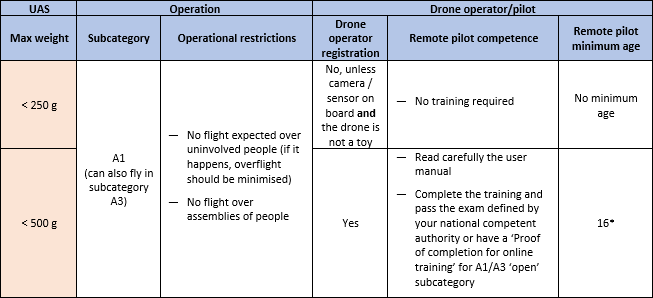
\includegraphics[scale = 0.9]{pictures/classification.PNG}
    \caption{Classification and restrictions for non-EASA class drones \cite{Euasa}}
    \label{fig:Table}
\end{figure}


When it comes to the state-of-the-art project, PULP-DroNet is a deep learning-powered visual navigation engine that enables autonomous navigation of a pocket-size quadrotor in a previously unseen environment. Thanks to PULP-DroNet the nano-drone can explore the environment, avoiding collisions even with dynamic obstacles, completely autonomously -- with no human operator and no ad-hoc external signals. This means that all the complex computations are done directly aboard the vehicle and very quickly. The visual navigation engine is composed of both a software and a hardware part. \cite{Niculescu2021}

When it comes to the future, the simulated pollination of agricultural plants by means of nano-copters could provide collecting and delivering pollen by means of autonomous control. A design of nano-copter for pollination can be made on the basis of innovative modifications of existing models by reprogramming flight controller that is to be fully adapted to computer interface. The robotic system is offered specially for artificial pollination in conditions of greenhouses and minor agricultural enterprises. \cite{Abutalipov2016}
